\documentclass{report}
\usepackage{graphicx} % Required for inserting images
\usepackage[italian]{babel}
\usepackage{tikz}
\usepackage{hyperref}
\usepackage{amsmath}
\usepackage{xcolor}
\usepackage{float}

\definecolor{darkgreen}{rgb}{0.0, 0.5, 0.0}


\title{DNA, Orecchio}
\date{Parte IX}

\begin{document}

\maketitle

\tableofcontents
\newpage

\chapter{DNA: uso nella biometria}

\section{Introduzione}

Le caratteristiche dei sistemi di riconoscimento degli individui 
basati sul DNA pongono questa metodologia come \textbf{la più
accurata nel panorama biometrico}.

\noindent Trova applicazioni in tanti ambiti:
\begin{itemize}
    \item biometrico
    \item medico 
    \item ambientale 
    \item ricerche storiche 
    \item forense
\end{itemize}

\noindent La \textbf{produzione di sensori allo stato solido} per analisi del DNA e la 
loro crescente diffusione fa prevedere nel futuro sempre più diffusione di sistemi
biometrici basati sul DNA ed in nuovi campi.

\noindent È una tecnica relativamente giovane: il DNA come identificativo biometrico 
è stato usato per la prima volta intorno al 1984.

\subsection{DNA e biometria}
Il DNA è un ottimo strumento di identficazione perché:
\begin{itemize}
    \item è presente in ogni cellula del nostro corpo in modo omogeneo
    \item la duplicazione cellulare (mitosi) duplica con estrema precisione il DNA 
    \item è una sequenza unica per ogni individuo:
    \begin{itemize}
        \item \textbf{solo dal 0,1\% al 0,5\% è diverso per ogni individuo}, il resto è uguale per tutti 
        \item questa porzione variabile è composta da milioni di coppie di basi (elementi costituenti del DNA)
    \end{itemize}
    \item è sufficiente una piccola porzione di campione per effettuare l'acquisizione del tratto
\end{itemize}


\section{Vantaggi e Svantaggi del DNA}

\begin{itemize}
    \item \textcolor{darkgreen}{\textbf{Vantaggi}}
    \begin{itemize}
        \item è la tecnica più accurata a disposizione 
        \item bastano poche cellule 
        \item è possibile scoprire una associazione tra sample di consanguinei
    \end{itemize}
    \item \textcolor{red}{\textbf{Svantaggi}}
    \begin{itemize}
        \item analisi non in real-time, servono alcuni minuti/ore 
        \item non è ancora completamente automatizzato 
        \item analisi costosa (da 100 fino a 2000 dollari)
    \end{itemize}
\end{itemize}



\section{Cos'è il DNA}
\begin{itemize}
    \item Il DNA ha una forma di doppia elica, si trova nel nucleo delle cellule
    \item È un polimero, ovvero una lunga molecola di unità di base (nucleotidi) ripetute;
    possono essere di 4 tipi:
    \begin{itemize}
        \item A (adenina)
        \item C (citosina)
        \item G (guanina)
        \item T (timina)
    \end{itemize}
    \item tutta l'informazione per generare un uomo è contenuta in una cellula, rappresentabile 
    come una sequenza di coppie
    \item il genoma umano è composto da circa \textbf{3 miliardi di coppie} (3 TB)
\end{itemize}

\subsection{Segmenti di DNA}

\noindent Le \textbf{coppie base} sono C-G/A-T, e si usano 
come unità di misura per contare la lunghezza di un \textbf{segmento} di DNA.

\begin{figure}[H]
    \centering
    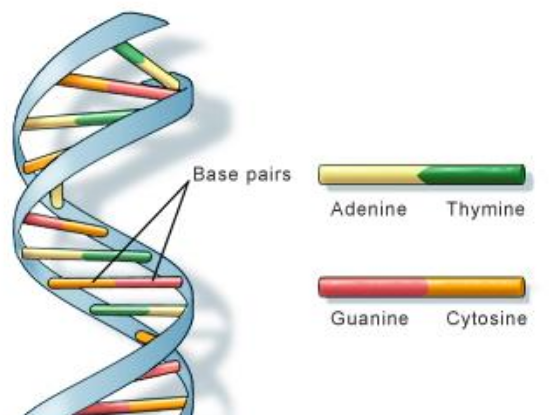
\includegraphics[width=0.6\linewidth]{images/elica.png}
\end{figure}


\subsection{Replicazione del DNA}
Se un intero individuo nasce da una cellula (embrione) e per 
tutta la sua vita in tutte le cellule vi è sempre la stessa 
molecola di DNA, significa che la \textbf{duplicazione del DNA è molto affidabile}. Il
processo naturale prende il nome di mitosi.

\noindent La \textbf{PCR} (\textit{Polymerase Chain Reaction}) è una tecnica che 
riesce a duplicare artificialmente delle piccole porzioni di DNA miliardi di volte 
in poche ore.

\subsection{Geni e alleli}
Ogni \textbf{gene} (porzione di 
DNA che ha informazioni su proteine o RNA) ha \textbf{fino 
a 100 versioni diverse, chiamati alleli}.


\section{Che feature si estraggono dal DNA}

Si potrebbe estrarre direttamente la sequenza di basi per un certo gene, ma sarebbe inutilmente troppo complesso.

\noindent In alcuni zone del DNA (\textit{locus}) ci sono dei \textbf{pattern di basi ripetuti},
ma ripetuti un \textbf{numero diverso} di volte per ogni individuo:

$\rightarrow$ \textbf{la vera feature biometrica quindi è il \underline{numero di 
ripetizioni} in un locus}

\noindent Con queste feature non è possibile scoprire malattie genetiche, \dots non è come 
avere tutte le informazioni di tutti i geni.

\subsection{DNA satellite}
Le porzioni di DNA che vengono ripetute prendono il nome di \textbf{satelliti}; si dividono 
in:
\begin{itemize}
    \item Macro satelliti ($>$ 100 coppie base)
    \item Mini satelliti (10-100 coppie base)
    \item Micro satelliti (2-7 coppie base), chiamati anche STR (\textit{Short Tandem Repeat})
\end{itemize}

\subsection{Quali dati mettiamo nel template}

L'FBI usa per il suo template:
\begin{itemize}
    \item 20 locus 
    \item \textbf{conteggia gli STR} 
\end{itemize}


\section{Estrazione del DNA}
\subsection{Dove trovare il DNA per le analisi}
\begin{itemize}
    \item sangue 
    \item sperma 
    \item saliva
    \item urina 
    \item capelli 
    \item denti 
    \item ossa 
    \item tessuti
\end{itemize}

\noindent È sufficiente una microscopica goccia di sangue o saliva per ottenere un campione 
valido per una analisi forense; normalmente si usa un campione di sangue o saliva.

\subsection{Fasi principali}
\begin{enumerate}
    \item \textcolor{blue}{\textbf{\textit{Collection}}}
    \item \textcolor{blue}{\textbf{\textit{Specimen storage}}}
    \item \textcolor{darkgreen}{\textbf{\textit{Extraction}}}
    \item \textcolor{darkgreen}{\textbf{\textit{Quantitation}}}
    \item \textcolor{darkgreen}{\textbf{\textit{PCR}}}
    \item \textcolor{orange}{\textbf{\textit{STR typing}}}
    \item \textcolor{orange}{\textbf{\textit{Interpretation of results}}}
    \item \textcolor{orange}{\textbf{\textit{Database storage \& searching}}}
    \item \textcolor{red}{\textbf{\textit{Probability of matching}}}
\end{enumerate}

\subsection{PCR per STR e contaminazioni}
\begin{itemize}
    \item La porzione di DNA che può essere amplificata è limitata, quindi si amplificano 
    solo i locus di interesse
    \item Gli STR che si usano sono \textit{estraibili} dal DNA con enzimi specifici
    \item L'amplificazione PCR è estremamente sensibile a contaminazioni
    \item La fase di \textbf{quantizzazione è fondamentale:}
    \begin{itemize}
        \item troppo poco DNA significa perdere degli alleli (una delle forme che può assumere un gene in un locus)
        \item troppo DNA provoca malfunzionamenti
    \end{itemize}
\end{itemize}

\subsection{Processo di estrazione}
\begin{itemize}
    \item Il DNA è un polimero carico elettrostaticamente, quindi viene attirato dai campi elettrici 
    \item Si possono separare dei segmenti di DNA in base alla loro lunghezza mettendoli in un gel posto in un campo elettrico 
    \item Ogni segmento di DNA, con lunghezza e carica diversa, si muove a velocità diversa (quelli con meno ripetizioni sono più veloci)
\end{itemize} 

\begin{figure}[ht]
    \centering
    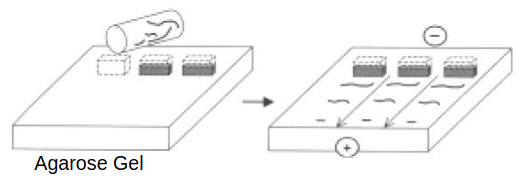
\includegraphics[width=0.8\linewidth]{images/estrazione.png}
\end{figure}

\newpage
\section{Matching}
Dai tracciati risultanti, i software per la genotipizzazione 
e l'esperto producono e controllano tutti i dati per il template 
da confrontare e/o memorizzare.

\begin{figure}[ht]
    \centering
    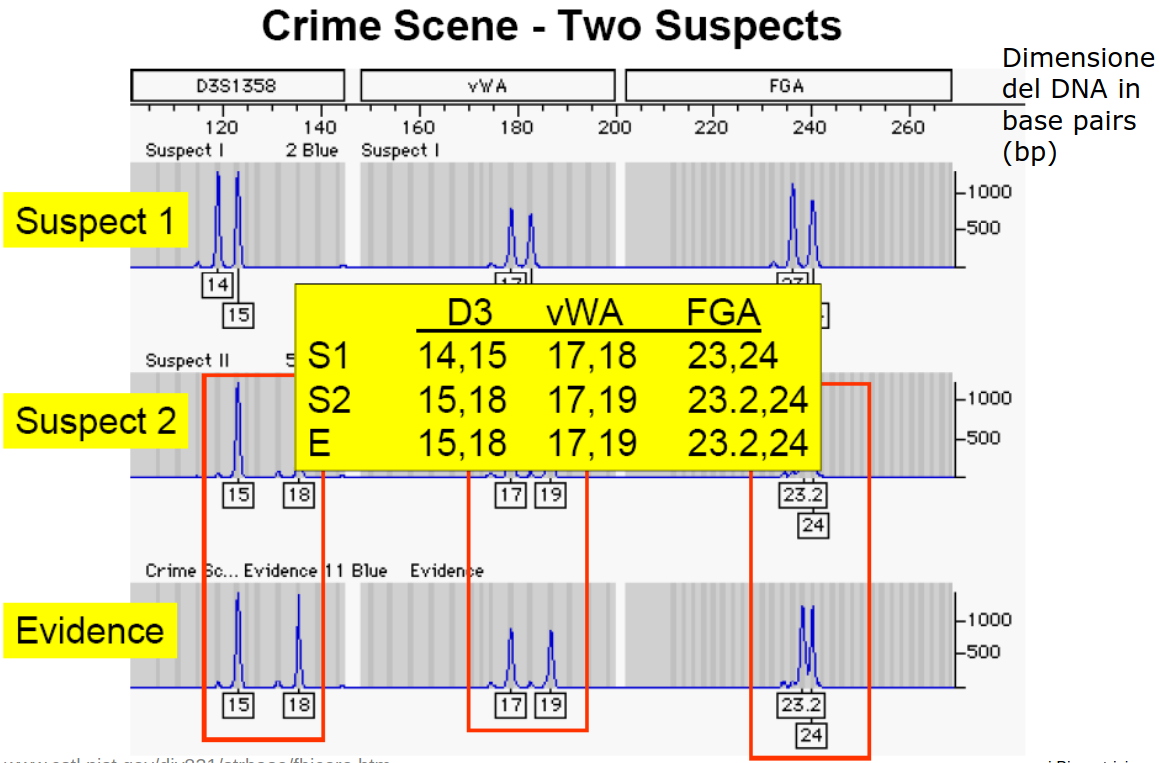
\includegraphics[width=1\linewidth]{images/matching.png}
\end{figure}

\noindent Bisogna fare attenzione ai problemi sperimentali 
che potrebbero causare falsi picchi di alleli o farli scomparire;
da questo punto di vista anche il DNA può sbagliare!

\subsection{Attenzione! Gemelli omozigoti}
Derivano da una singola cellula uovo fecondata da uno spermatozoo;
al concepimento hanno lo stesso DNA. Tuttavia, durante lo sviluppo possono intervenire mutazioni
somatiche che vanno a differenziare il DNA.

\noindent Solo pochi laboratori capaci di analisi molto avanzate
trovano in modo affidabile le piccolissime differenze
del DNA degli omozigoti.

\newpage
\section{Problemi di privacy}
\begin{itemize}
    \item \textit{Mandando il DNA ad una azienda per l'analisi, si possono rintracciare i parenti 
    dato che \textbf{contengono le stesse porzioni DNA}}

    $\rightarrow$ il problema è che vengono esposti anche i discendenti nel futuro! 
    \item 1 solo individuo espone più di 1000 persone al tracciamento
    \item oltre alla possibilità di essere riconosciuto, il DNA rivela dati su malattie e predisposizioni \dots
    informazioni sensibili!
\end{itemize}

\noindent Usando dati pubblici è stato creato un albero genealogico di 13 milioni di individui.


\chapter{Orecchio}

\section{Perché? Vantaggi e Svantaggi}

\begin{itemize}
    \item \textcolor{darkgreen}{\textbf{Vantaggi}}
    \begin{itemize}
        \item tratto spesso nascosto $\rightarrow$ difficile da copiare, privacy compliant
        \item non si conoscono attacchi realistici su questo tratto 
        \item usabile quando il volto è laterale e non funzionano i sistemi classici
        \item implementabile su molti device (cellulare, webcam)
    \end{itemize}
    \item \textcolor{red}{\textbf{Svantaggi}}
    \begin{itemize}
        \item non standard (no ISO, \dots)
        \item occlusioni
        \item non sempre applicabile
    \end{itemize}
\end{itemize}

\begin{figure}[H]
    \centering
    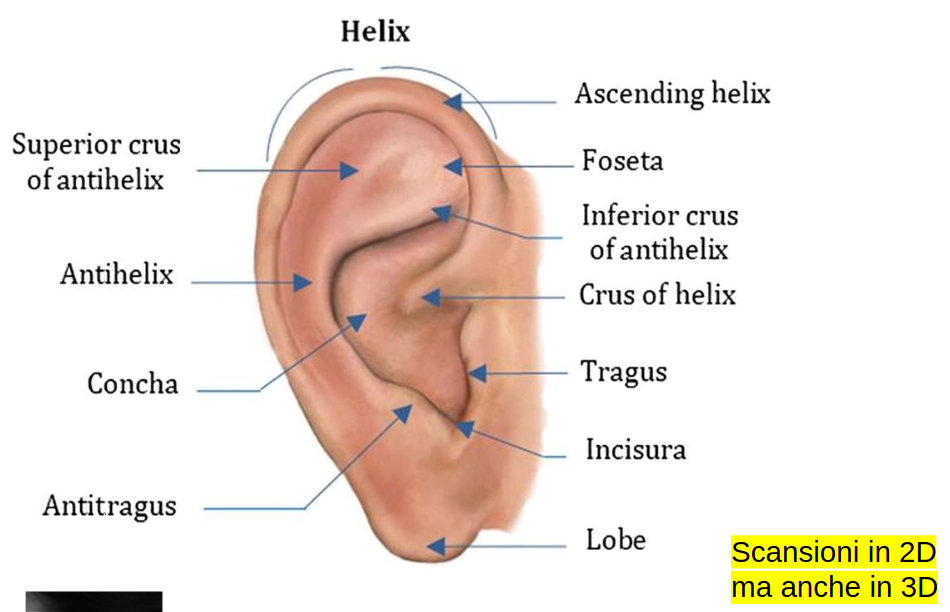
\includegraphics[width=0.8\linewidth]{images/orecchio.png}
\end{figure}

\section{Estrazione delle feature}

\subsection{Eigenears (come autofacce)}
\begin{figure}[H]
    \centering
    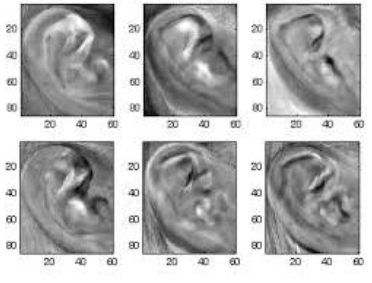
\includegraphics[width=0.8\linewidth]{images/eigenears.png}
\end{figure}

\subsection{Estrazione mediante contorni}
\begin{figure}[H]
    \centering
    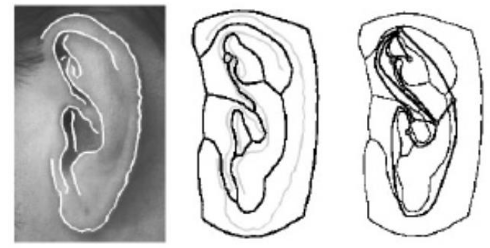
\includegraphics[width=0.8\linewidth]{images/contorni.png}
\end{figure}

\newpage
\subsection{Distanze dal centro dei punti principali}
\begin{figure}[ht]
    \centering
    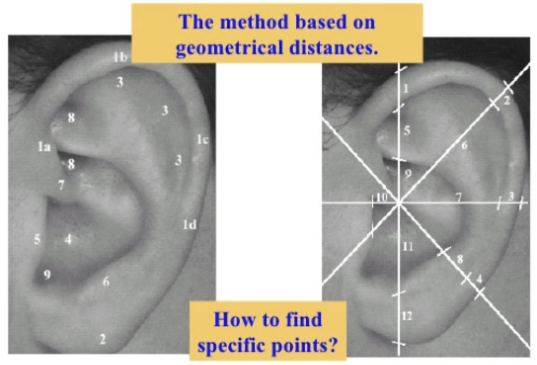
\includegraphics[width=0.9\linewidth]{images/punti.png}
\end{figure}

\noindent Non semplice e ben automatizzabile
selezionare i punti specifici.

\newpage
\section{In caso fosse sfuggito qualcosa \dots}
\begin{figure}[H]
    \centering
    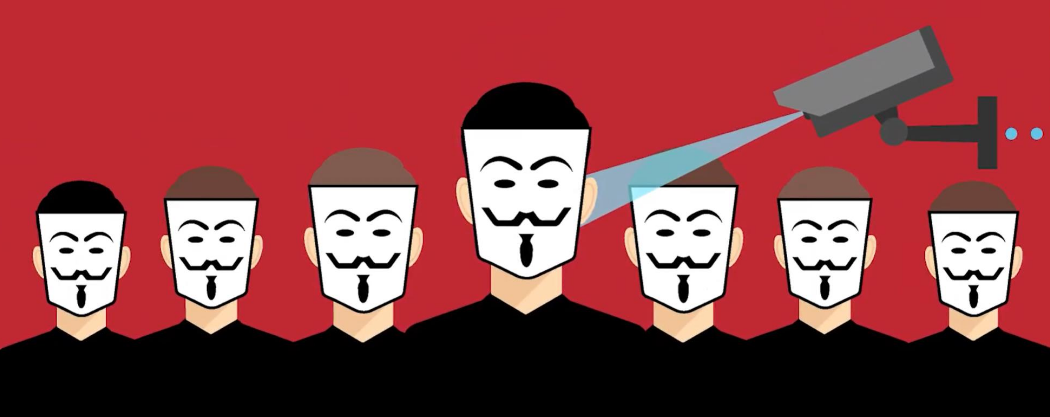
\includegraphics[width=1\linewidth]{images/orecchio-applicazione1.png}
\end{figure}

\begin{figure}[H]
    \centering
    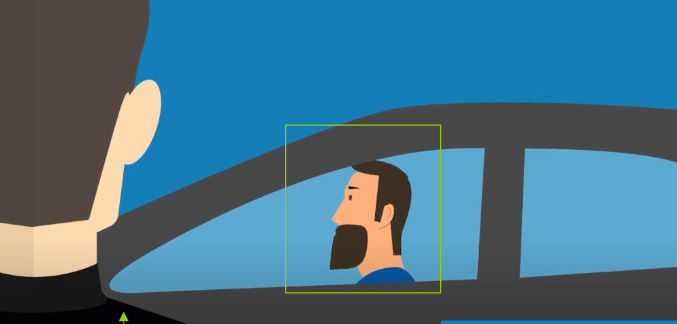
\includegraphics[width=1\linewidth]{images/orecchio-applicazione2.png}
\end{figure}

\begin{itemize}
    \item Volto parzialmente occluso, riflessi, vista laterale, \dots
    \item È un tratto che può essere usato con i sistemi multimodali, e che entra in funzione 
    quando gli altri smettono
\end{itemize}


\end{document}